\chapter{Experiments}
We denote the combination of an image representation with a classifier by \emph{representation/classifier} (for example, the \dtcwt{} combined with a Random Forest is denoted by \dtcwt{}/RF).

These learning variants were developed for two reasons: firstly, when analyzing quantitative results for detection performance, they allow us to decouple the effect of random forest learning from the effect due to the type of representation used. 


\section{Datasets}
\subsection{Real Mammograms}
The main purpose of this work was to develop methods for analysing curvilinear structure in mammogram images. To evaluate the algorithms, we took images from a sequential set of 84 abnormal mammograms with biopsy-proven malignancy, drawn from a screening population (Nightingale Breast Centre, South Manchester University Hospitals Trust, UK), and from a set of 89 normal mammograms of the contralateral breasts of the same individuals (where disease was radiologically confirmed to be confined to one breast). All mammograms were digitised to a resolution of $90 \mu\text{m}$ using a Vidar CADPRO scanner. A $4 \by 4$ cm ($512 \by 512$ pixel) patch was then extracted around each abnormality, and a similar patch sampled randomly from each of the normal mammograms (\fref{f:real_examples}). 

For each abnormal patch, an expert radiologist manually annotated some (though not necessarily all) of the spicules associated with the abnormality, giving a total of 555 spicule annotations. Though these expert spicule annotations were not sufficiently accurate to be used directly, we used them as a basis for selecting spicule pixels by initialising a snake~\cite{Kass_etal_IJCV88} with each original annotation, and iterating it to convergence using evidence from the\comment{linear structure probability} image~\cite{Muralidhar_etal_TMI10}. In total, the 555 refined spicule annotations identified 36\,514 spicule pixels. To ensure balanced training sets, we sampled the same number from the normal images.


\subsection{Synthetic Mammogram-like Images}
Given the practical difficulties of obtaining a precise binary labelling of curvilinear structure in mammograms, we generated synthetic images with which to train and evaluate each algorithm\cite{Berks_PhD10}. Specifically, to create each image we again took a $4 \by 4$ cm ($512 \by 512$ pixel) region from a real mammogram with 256 grey levels, and processed it\comment{be more specific} to remove linear structures, leaving only the coarse background texture with local image noise across all frequencies. We then superimposed several linear structures with randomly chosen parameters (orientation, width, peak intensity, \comment{curvature,?} profile shape, etc) onto the background. The result was an image whose statistics were close to a real mammogram but with known line parameters (\fref{f:synthetic_responses}).

In this manner, we generated 10\,460 training images and 4\,903 test image patches from 72 (30) normal mammograms. The line parameters were drawn from probability distributions that were chosen to mimic what is found in real mammograms:

\begin{itemize}
\item orientations were drawn from a uniform distribution over the range [0, $\pi$] radians.
\item widths were drawn from a uniform distribution over [4, 16] pixels.
\item peak intensity [1,255] grey-levels (relative to images scaled 0 - 255) from an exponential distribution with half-width 4 grey-levels; 
\item profile shape $S$ determined by the equation $S = s + (1-s) \sin(x)$ for offsets $x \in (0,\pi)$, where the 'squareness' parameter $s$\comment{could be confused with scales defined elsewhere} determines how close the shape is to a pure half-cycle $\sin$ or a rectangle and is drawn uniformly from [0,1]. 
\end{itemize}

The literature suggests (and this is borne out by our experience) that the best performance is obtained by training with a balanced dataset - in this case with the same number of foreground (curvilinear structure) and background examples. Having created these images, therefore, we sampled feature vectors at pixels on the centrelines of the superimposed linear structure, and an equal number of `background' pixels to serve as positive and negative training sets, respectively.\comment{for detection, of course} 

When testing an algorithm on an unseen image, we compute the output for every pixel in the image.

To construct the orientation regression random forests, we sample points randomly from line pixels in the synthetic images (the orientation of a background pixel is undefined).

During training, backgrounds were randomly sampled from the 10460 training patches and a single line was added to the centre of the patch. These images were produced 'on-the-fly' during each tree-building step of random forest construction and no permanent set was maintained. (We simply generated images until we had the desired 200k points, then built the tree; we did this for 200 trees.)

For testing, 100 backgrounds were randomly selected from the test patches. To each, multiple lines were added sequentially, with the number and position of lines varying randomly.

Note that all synthetic lines used were straight lines. We conducted experiments explicitly using curved structures, however as there was no performance difference between training on curved or straight lines when detecting curved lines, it was decided that including curves was unnecessary.

All forests were constructed with 200 trees and following published guidelines~\cite{Breiman_ML01}. However, rather than using a single set of training data from which samples were drawn with replacement (\ie bootstrapping), we used our method for randomly generating unique synthetic lines images to construct a new training sample at each tree-building step. For detection, each sample comprised 100k curvilinear structure pixels and 100k background pixels, while for orientation regression we used 200k pixels all belonging to curvilinear structure. 


\subsection{Retinal Images}
The publicly available DRIVE dataset~\cite{Staal_etal_TMI04} contains 40 full colour retinogram images (\fref{f:retinography}a) of $565 \by 584$ pixels, each with a hand-labelled mask that indicates vessel pixels (\fref{f:retinography}b), and split into training (images 21-40) and test (images 01-20) sets. The masks provided ground truth for the presence of a line in the image, and by skeletonizing the mask we approximated ground truth orientation, $\theta_{gt}$, for every labelled pixel.\comment{It is questionable how well this constitutes ground truth}

For training, we transformed all images to monochrome via a weighted sum of the three RGB channels (though using only the green channel is also popular). We then selected 200\,000 vessel pixels randomly over the training set and computed filter responses for every selected pixel.

\begin{figure}[t]
\centering
\begin{tabular}{c c c}
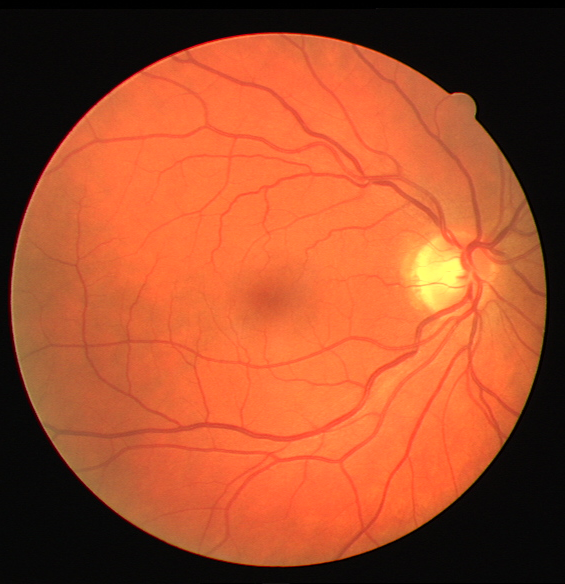
\includegraphics[width=0.3\columnwidth]{\figpath/retina/02_test} &
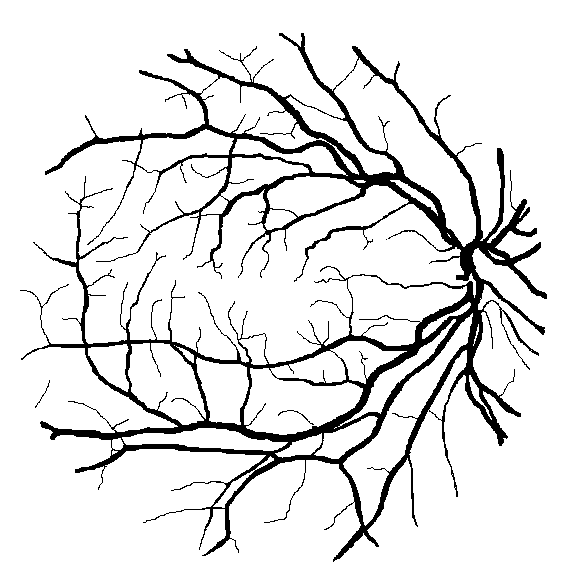
\includegraphics[width=0.3\columnwidth]{\figpath/retina/02_manual1} &
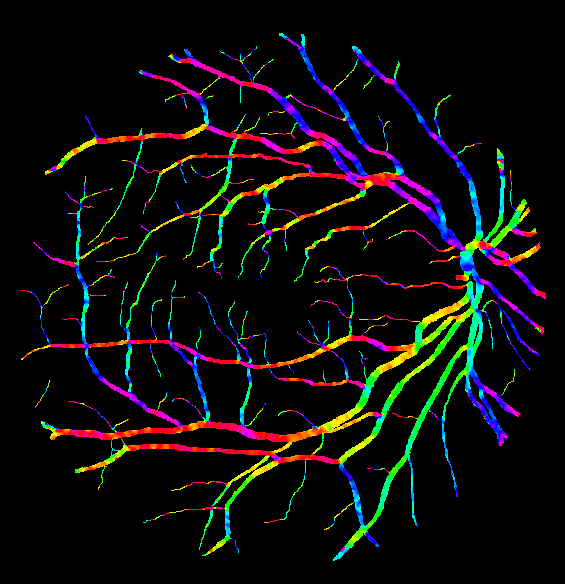
\includegraphics[width=0.3\columnwidth]{\figpath/retina/002_orientation_masked} \\
%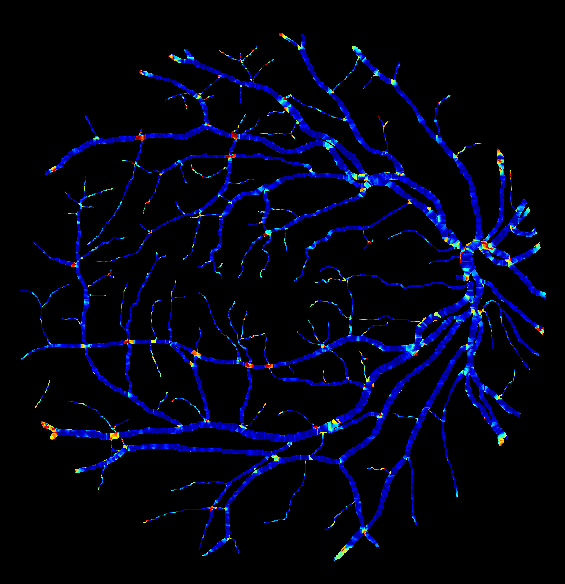
\includegraphics[height=0.15\textheight]{\figpath/retina/002_abs_error} \\
(a) & (b) & (c) \\
\end{tabular}
%
\caption{Estimating orientation in retinography: %
(a) input image; %
(b) ground truth mask indicating pixels belonging to a vessel; %
(c) orientation (indicated by colour) estimated using linear regression over \dtcwt{} features. The mask was not used to estimate orientation. %
%(c) magnitude of error (note the regions of high error at points of bifurcation.)
}
\label{f:retinography}
\end{figure}


\subsection{Fingerprint Images}
\comment{Where did this data come from?}
Noting that estimating orientation is of interest to the fingerprint analysis community, we briefly present some results that highlight the difference in performance between using filters based on first and second derivatives, respectively. As discussed earlier, the estimated orientation using gradient based filters~\cite{Bazen_Gerez_TPAMI02,Mei_etal_IVC09} -- the mainstay of fingerprint orientation analysis -- becomes unstable near the centre of a symmetric bar feature (\fref{f:fingerprints}c), whereas a filter based on second derivatives remains stable. There are, however, artefacts around the edges of the ridge features for the second derivative that may suggest a solution based on both types.

\begin{figure}[t]
\centering
\begin{tabular}{c c c}
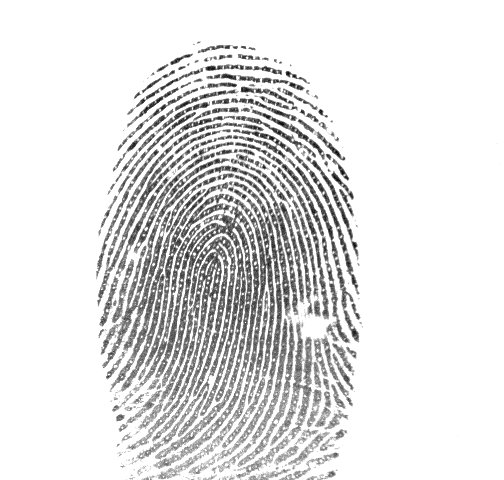
\includegraphics[width=0.3\columnwidth]{\figpath/fingerprint/input} &
%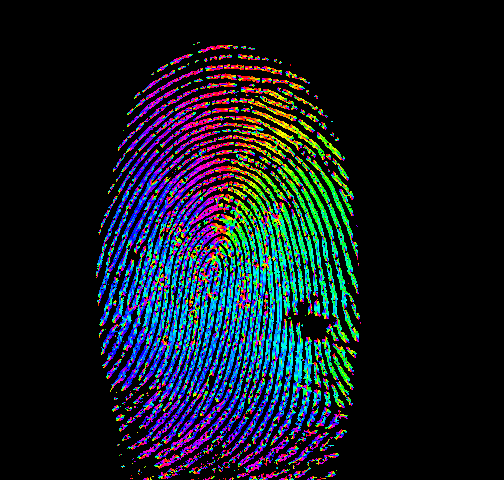
\includegraphics[height=0.15\textheight]{\figpath/fingerprint/ori_1st} &
%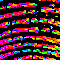
\includegraphics[height=0.15\textheight]{\figpath/fingerprint/ori_1st_zoom} \\
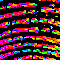
\includegraphics[width=0.3\columnwidth]{\figpath/fingerprint/ori_1st_zoom} &
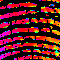
\includegraphics[width=0.3\columnwidth]{\figpath/fingerprint/ori_clover_zoom} \\
(a) & (b) & (c) \\
%&
%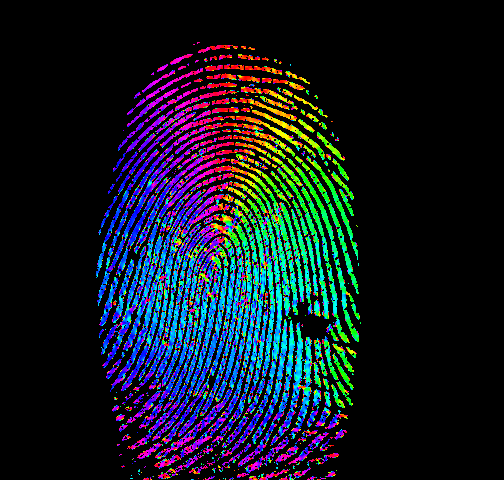
\includegraphics[height=0.15\textheight]{\figpath/fingerprint/ori_clover} &
%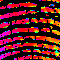
\includegraphics[height=0.15\textheight]{\figpath/fingerprint/ori_clover_zoom} \\
%		& (d) & (e)
\end{tabular}
%
\caption{Fingerprint images: %
(a) input image; %
(b,c) first derivative estimate of orientation with close-up; %
(d-e) second derivative estimate with close-up. Note the high errors at the centre of the ridge for first derivatives and at the edges of the ridge for second derivatives.}
\label{f:fingerprints}
\end{figure}


\subsection{Nailfold Capillaroscopy Images}



\section{Detecting Linear Structures}
In our first set of experiments, we investigate the ability of each image representation and classification method to detect the presence of a line (\ie~a bar) in the image. For this task, we used a binary label (present \vs not present) as the target we aimed to predict.

Having trained a classifier using the synthetic data, we can classify feature vectors extracted about every pixel in a synthetic or real mammogram image to obtain a line probability image (using the probabilistic labelling scheme as opposed to a hard binary classification).

Monogenic, Linop and Gaussian are representative of the current state of the art in line detection, and all permit an analytic approach to line detection.

Secondly, unlike their original variants, Monogenic/RF, Linop/RF and Gaussian/RF can be used in the spicule classification experiment.

By forming such a feature vector at each pixel in a training set of ground-truth labelled images, we can obtain a large set of data which can be used to train a random forest classifier to differentiate between linear structures and background. In constructing the best detector, this discriminative approach takes account of the characteristics of the background pixels as well as the curvilinear structure pixels.

Details on the composition of feature vectors for each representation type are given below. Note for all methods, the number of scales used $s$ and the neighbourhood size $w$ were empirically tested to select the best combination for each method. In each case, we tried $s$ = 3, 4, 5, 6 and $w$ = 1, 3. For reasons of space, results are shown only for the best combination in each method.

\begin{itemize}
\item	DT-CWT/RF: images were decomposed using the DT-CWT to $s$ scales. Neighbourhoods of interpolated phase and magnitude coefficients were extracted in each of the 6 oriented subbands producing a feature vector of $12 w^2 s$ elements.
\item	Monogenic/RF: the monogenic signal was extracted across $s$ scales, with the initial wavelength set at $\lambda$ = 4 pixels. Neighbourhoods of phase, amplitude and orientation values were computed giving a total feature size of $3 w^2 s$. 
\item	Linop/RF: 8 oriented line filters were computed at each scale. Collecting neighbourhoods of the oriented filter responses produced $8 w^2 s$ elements in each feature vectors.
\item	Gaussian/RF: for the Gaussian 2nd derivative method, the three directional derivatives were applied to an image at each scale. The standard deviation of the smallest kernel was 1 pixel, subsequent kernels increased by a factor of 2 at each scale. As with Monogenic/RF this resulted in feature vectors with $3 w^2 s$ elements.
\end{itemize}

For testing, feature vectors for each representation were extracted at all pixels in the 100 synthetic test images. The classification and regression forests were then used to compute a line detection score (the proportion of votes for the curvilinear structure class) . Example results of line detection are shown in~\ref{f:synthetic_responses}.


\begin{figure}
\centering
\begin{tabular}{c c c c}
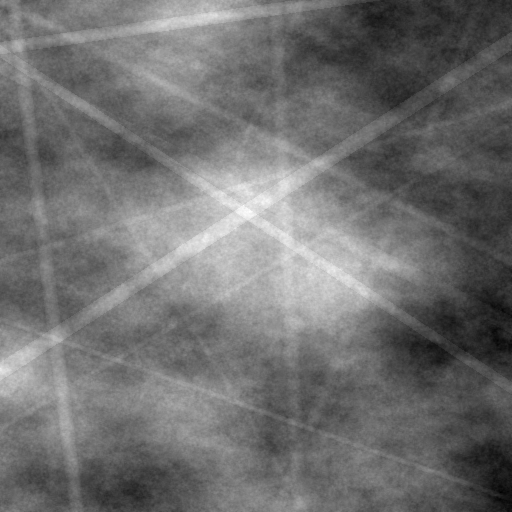
\includegraphics[width=\qtrcol]{\figpath/ipmi/line512_003} &
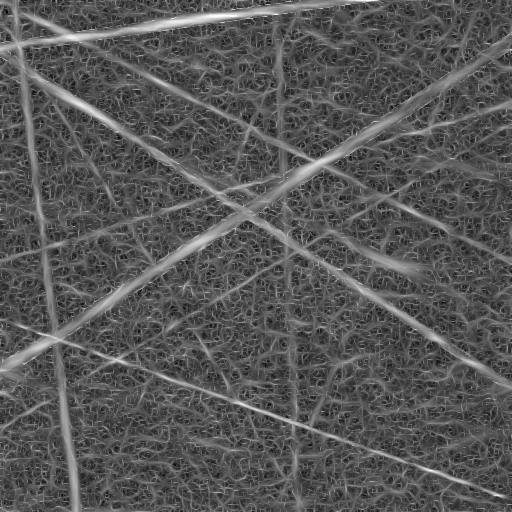
\includegraphics[width=\qtrcol]{\figpath/ipmi/line512_003_lines} &
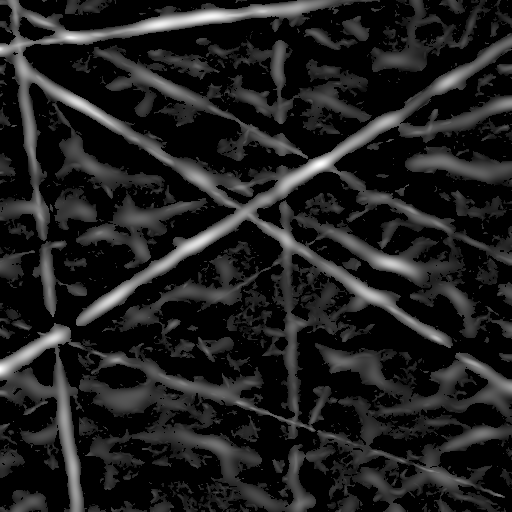
\includegraphics[width=\qtrcol]{\figpath/ipmi/line512_003_gaussian} &
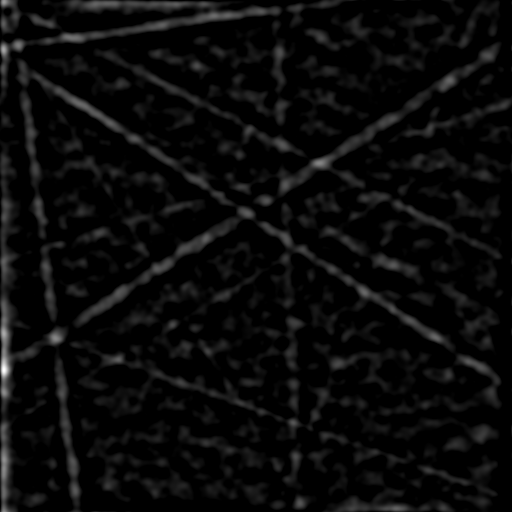
\includegraphics[width=\qtrcol]{\figpath/ipmi/line512_003_monogenic} \\
(a) & (b) & (c) & (d) \\
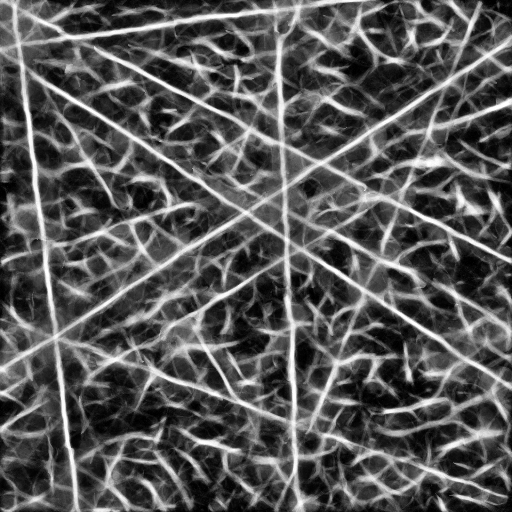
\includegraphics[width=\qtrcol]{\figpath/ipmi/line512_003_rf_191905} &
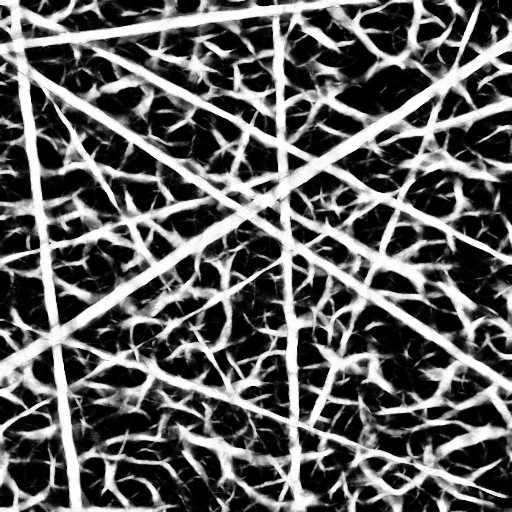
\includegraphics[width=\qtrcol]{\figpath/ipmi/line512_003_rf_191961} &
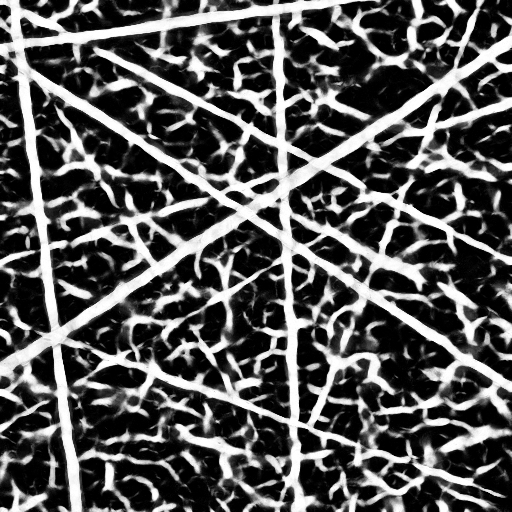
\includegraphics[width=\qtrcol]{\figpath/ipmi/line512_003_rf_233141} &
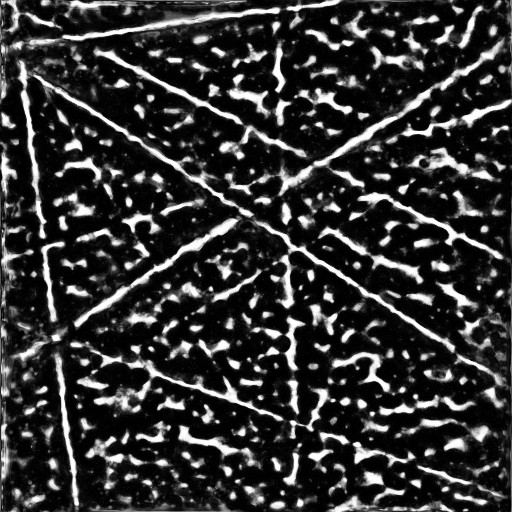
\includegraphics[width=\qtrcol]{\figpath/ipmi/line512_003_rf_191960} \\
(e) & (f) & (g) & (h)
\end{tabular}
%
\caption{Synthetic test image and corresponding filter responses: (a) original image; (b) Linop; (c) Gaussian; (d) Monogenic; (e) DT-CWT/RF; (f) Linop/RF; (g) Gaussian/RF; (h) Monogenic/RF.}
\label{f:synthetic_responses}
\end{figure}


\begin{figure}
\centering
\begin{tabular}{c c c c}
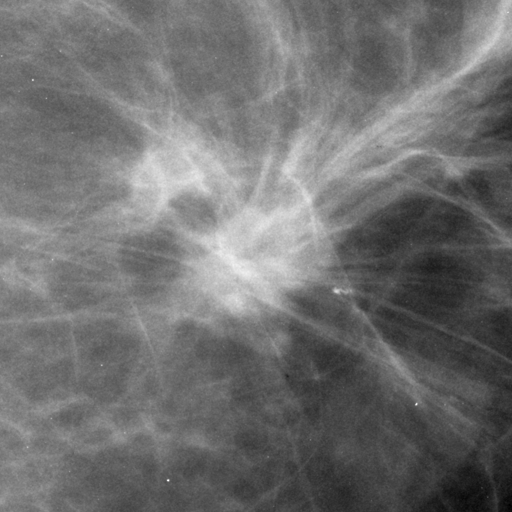
\includegraphics[width=\qtrcol]{\figpath/ipmi/mass028} &
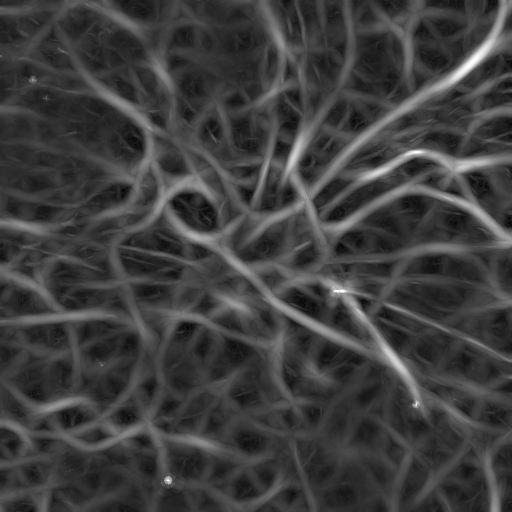
\includegraphics[width=\qtrcol]{\figpath/ipmi/mass028_linop} &
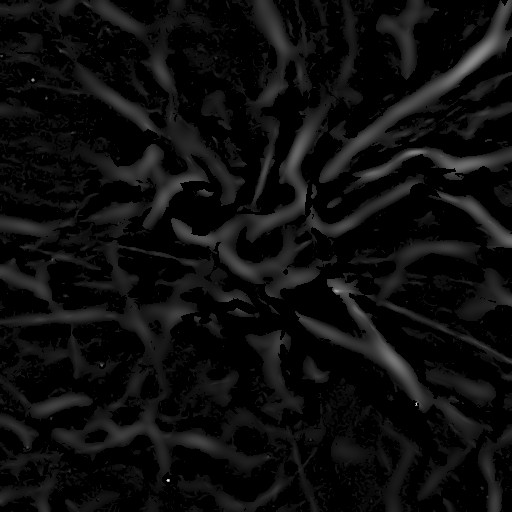
\includegraphics[width=\qtrcol]{\figpath/ipmi/mass028_gaussian} &
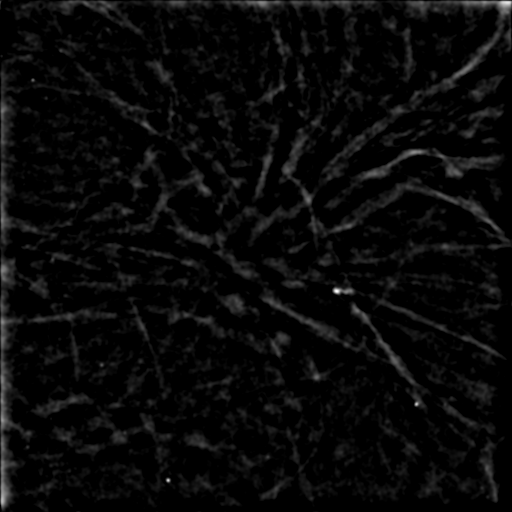
\includegraphics[width=\qtrcol]{\figpath/ipmi/mass028_monogenic} \\
(a) & (b) & (c) & (d) \\
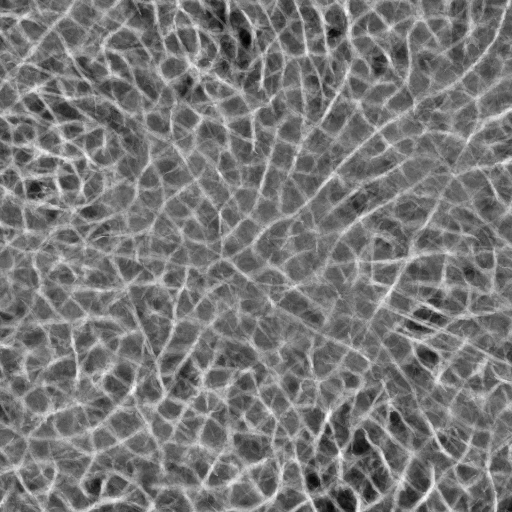
\includegraphics[width=\qtrcol]{\figpath/ipmi/mass028_dt} &
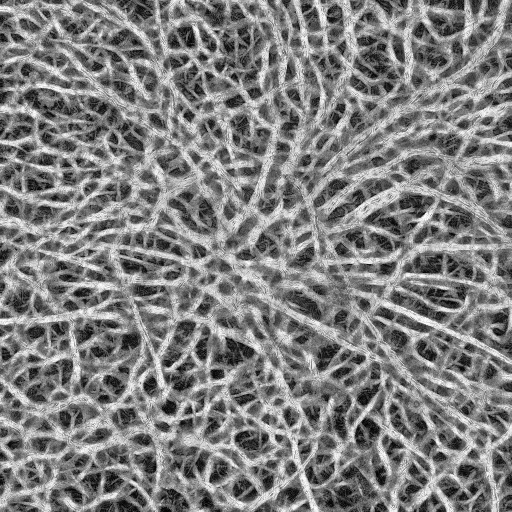
\includegraphics[width=\qtrcol]{\figpath/ipmi/mass028_rf_linop_w1l5} &
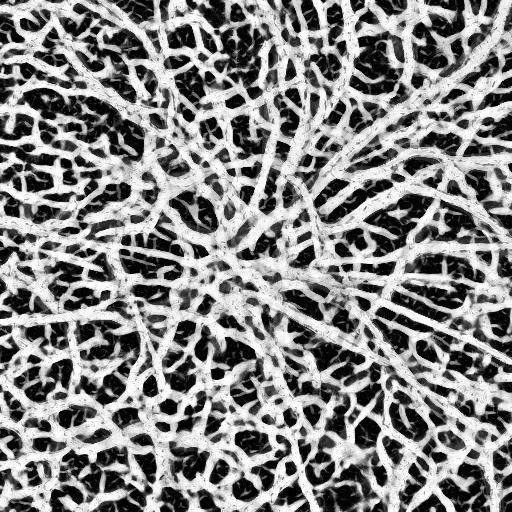
\includegraphics[width=\qtrcol]{\figpath/ipmi/mass028_rf_gaussian} &
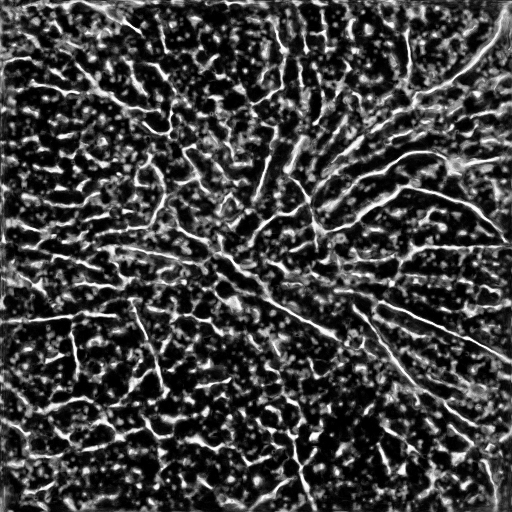
\includegraphics[width=\qtrcol]{\figpath/ipmi/mass028_rf_monogenic_w3l4} \\
(e) & (f) & (g) & (h)
\end{tabular}
%
\caption{Mammogram region containing malignant spiculated mass and corresponding filter responses: (a) original image; (b) Linop; (c) Gaussian; (d) Monogenic; (e) \dtcwt{}/RF; (f) Linop/RF; (g) Gaussian/RF; (h) Monogenic/RF.}
\label{f:real_responses}
\end{figure}


\begin{figure}
\centering
\begin{tabular}{c c c}
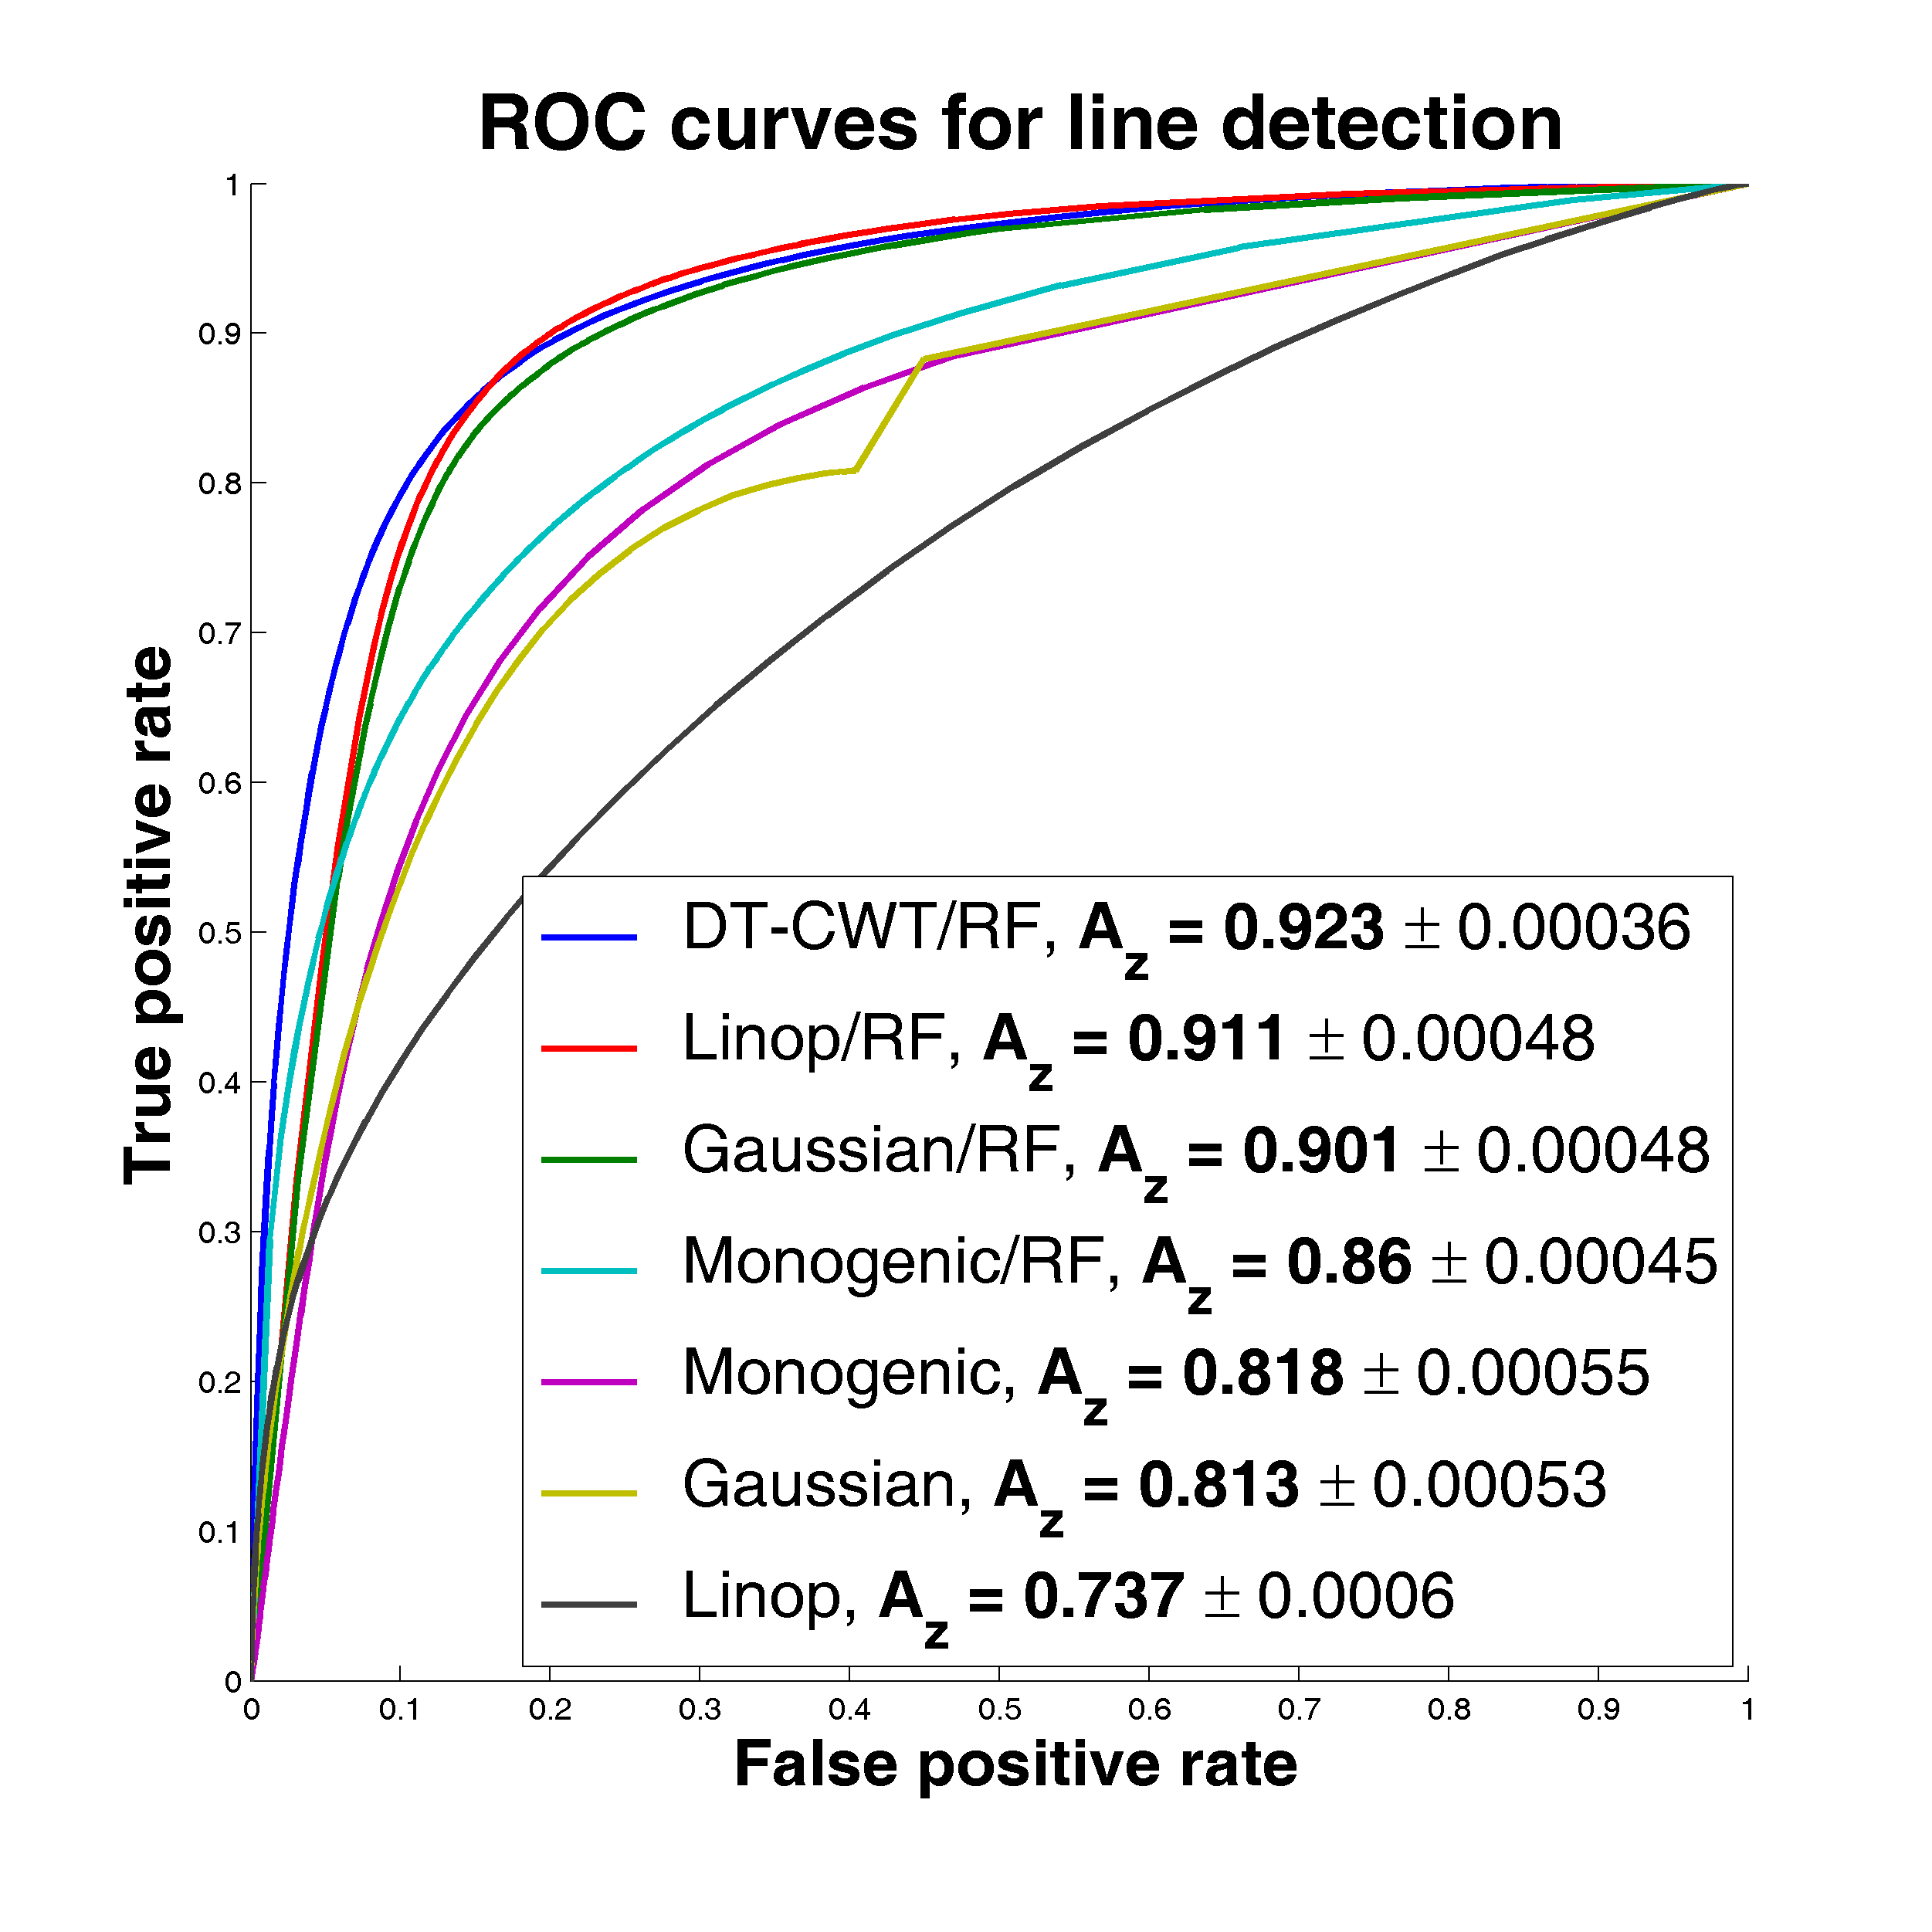
\includegraphics[width=0.33\columnwidth]{\figpath/ipmi/line_detection_roc} &
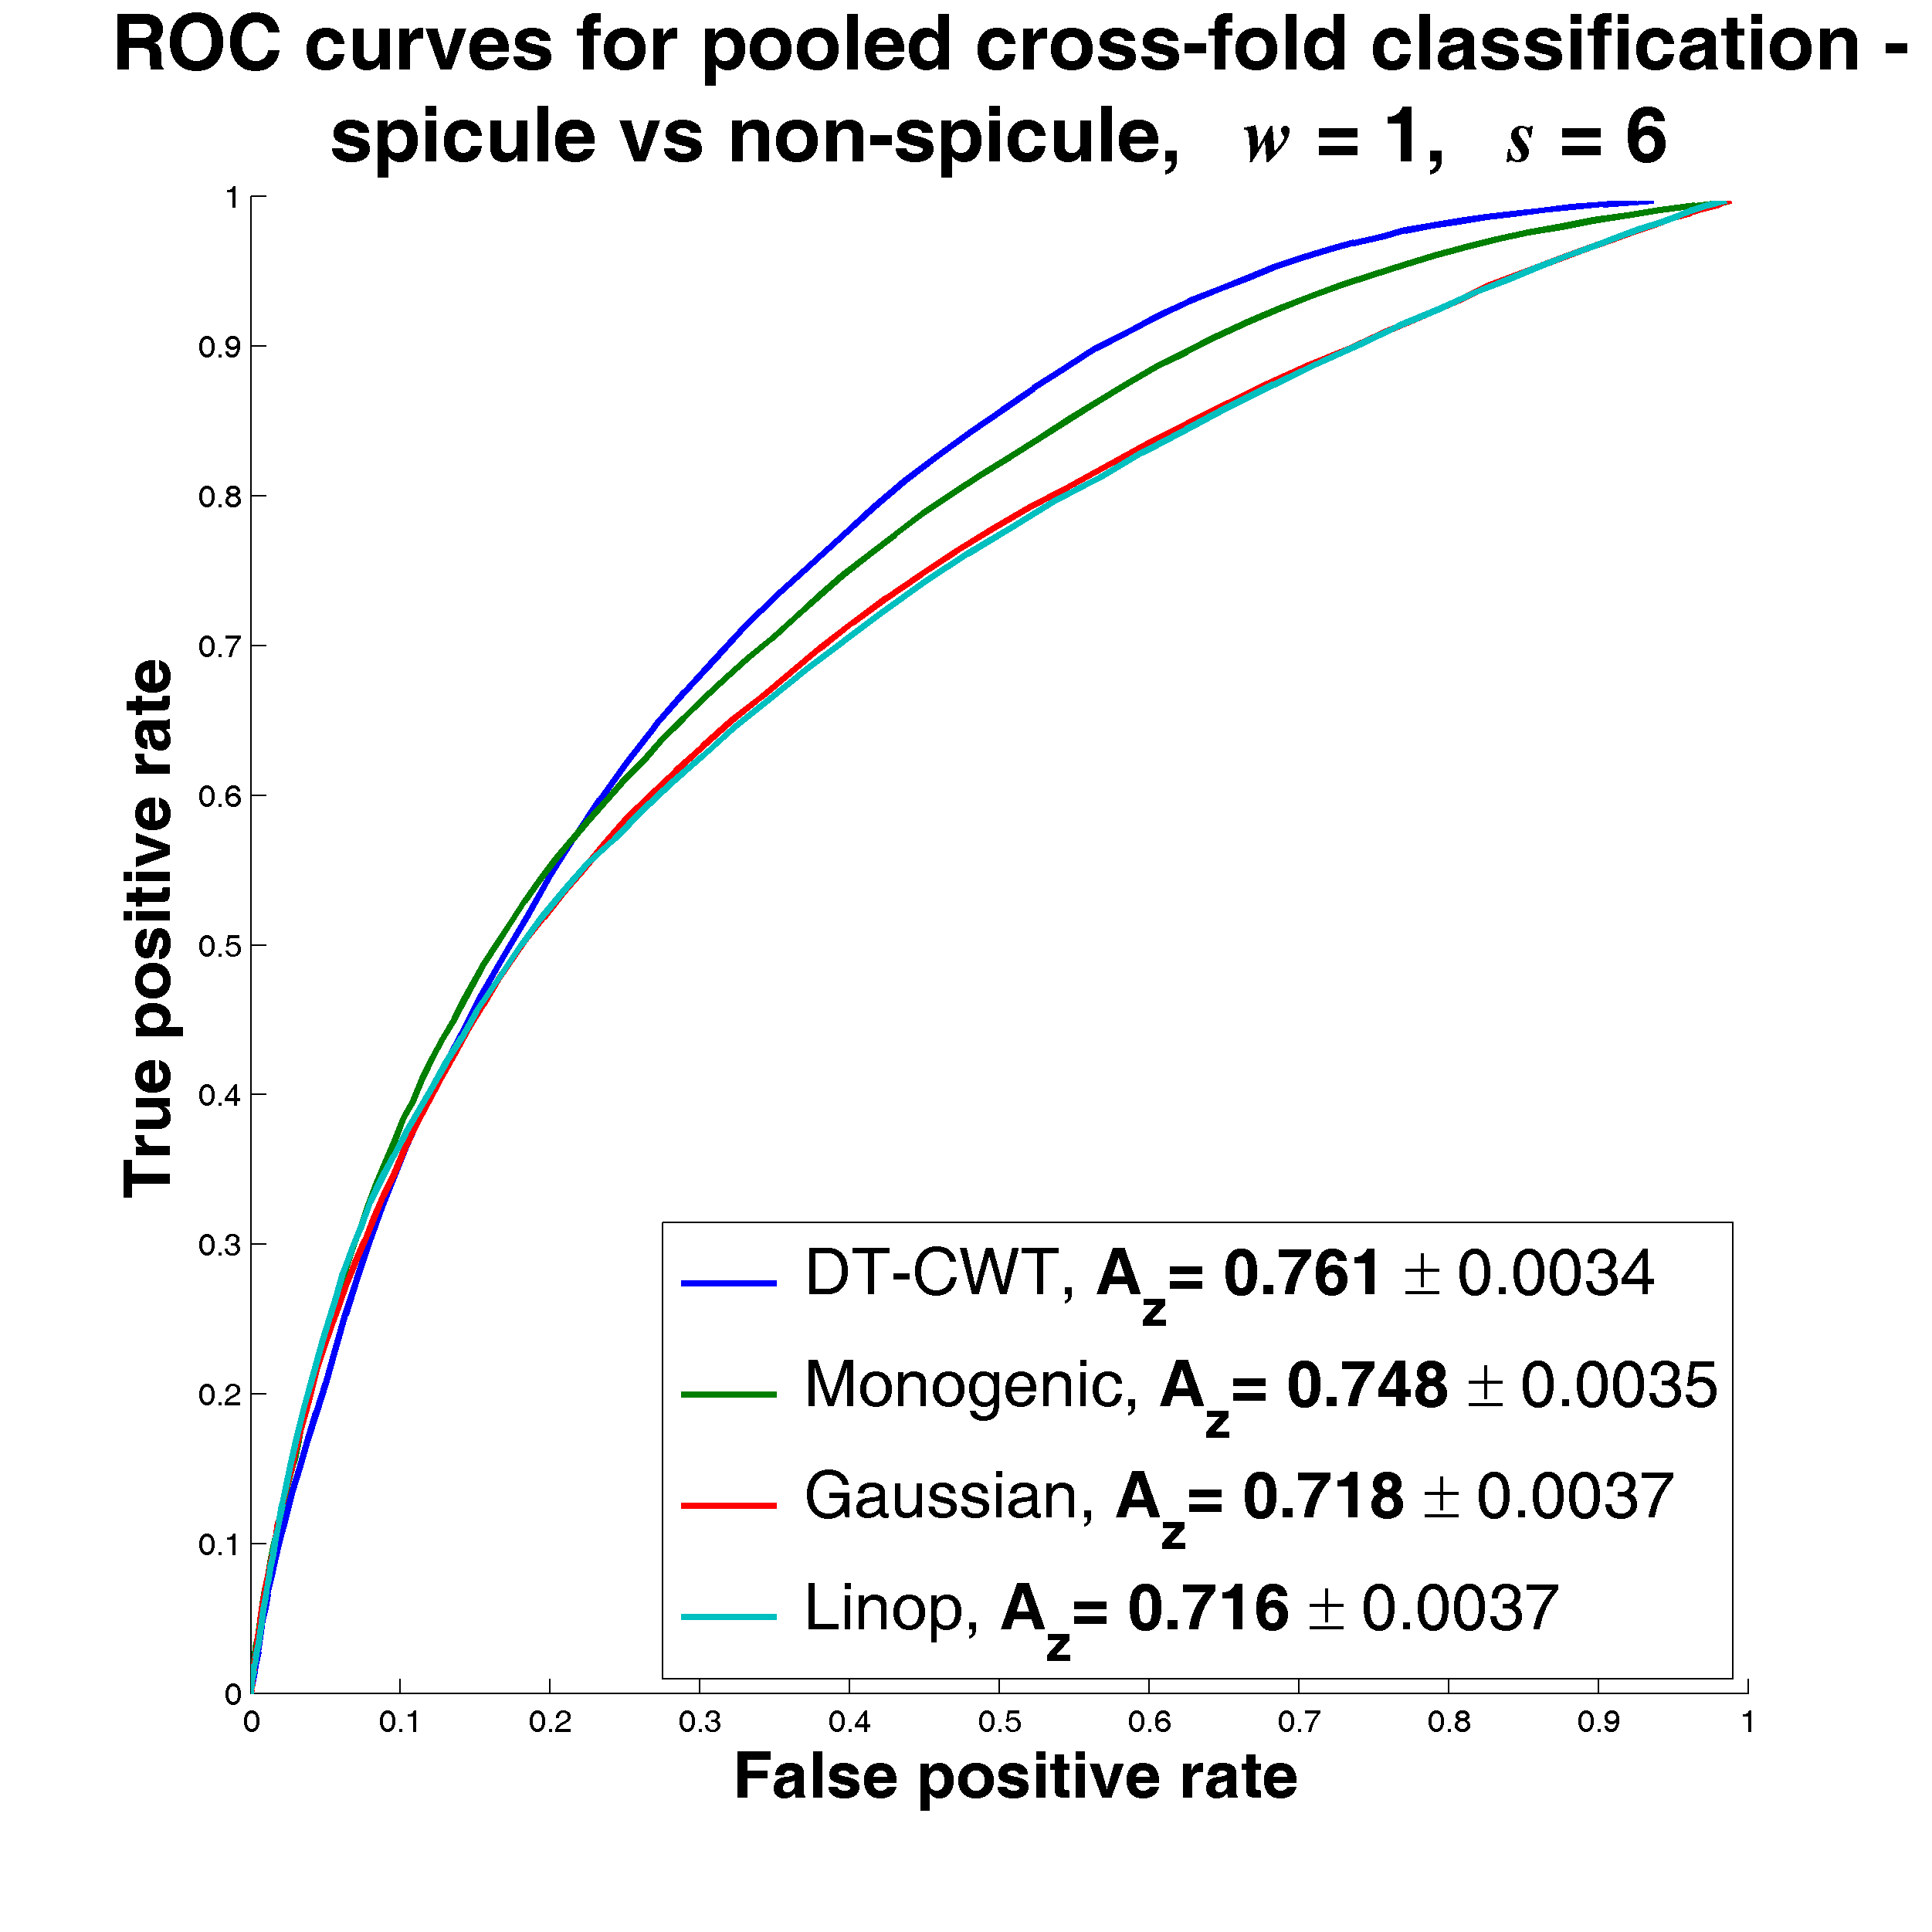
\includegraphics[width=0.33\columnwidth]{\figpath/ipmi/rf_spic_1_6}
\end{tabular}
%
\caption{Receiver operating characteristic (ROC) curves for different curvilinear structure detection methods; centre: Cumulative distribution functions (CDF) of errors in orientation estimation for the different methods; right: ROC curves for spicule classification.}
\label{f:detection_roc}
\end{figure}

ROC curves for the seven methods tested are shown in~\ref{f:} 2, using the known ground-truth for the test images to define pixels on the centrelines of curvilinear structures as foreground, and pixels lying outside the structures as background. Areas under the ROC curves and detection sensitivities at a fixed specificity of 90\% are shown in~\ref{t:}. 

These results show that the four learning methods perform significantly better than the three prescriptive methods (with the exception of orientation computation in Monogenic/RF). \dtcwt{}/RF is significantly the strongest performing for both line detection and orientation estimation, followed by Linop/RF then Gaussian/RF.

As expected, because Linop, of the three prescriptive methods, discards the highest proportion of filter responses, Linop/RF gains the most from training. This highlights the ability of the random forests to extract useful information from a rich local description of image content, and while we do not have a prescriptive variant to compare it to, we believe this shows the importance of training in maximizing the benefit of using the \dtcwt{}. We also note that the added information that can be gained from the \dtcwt representation results from an increase in the richness of the local description of texture and is not due to increasing the support of the descriptor. Indeed, as described above we tested all representations over an equivalent range of filter scales so that the same image support was available to each method.

Assessing the detection results visually, it would appear that the outputs of the learning based methods (and particularly \dtcwt{}/RF, Linop/RF and Gaussian/RF) are similar to the output of synthetic data while capturing the key curvilinear structures in the real regions. This would suggest our model for producing synthetic lines generates good data from which to train random forests for real images. Of course validating this hypothesis is important and we are currently working on a quantitative evaluation of the methods in real data when used, for example, as part of a larger lesion detection scheme.


\section{Classifying Linear Structures}
Classification is of interest when it is important to distinguish between subtly different structures which may be present within the same image - for example, rivers and roads

When classifying between different types of linear structure, our hypothesis is that the cross-sectional intensity profiles of different structures vary in systematic ways~\cite{Zwiggelaar_etal_TMI04} that can be used to discriminate between classes.

, and that profile shape is effectively captured by the \dtcwt{} coefficients - particularly in the phase components. 

We concentrated on the task of distinguishing between spicules (an indicator of malignancy) and other curvilinear structures.  To create a balanced training set we sampled feature vectors from the same number of pixels in a set of normal mammogram patches, such that the distribution of curvilinear structure probabilities was the same as for the spicule training set. Using this balanced training set, we built a random forest classifier to perform spicule/non-spicule classification.

The literature on classifying curvilinear structures in mammograms is much more limited. We are aware of the work of Zwiggelaar et al~\cite{Zwiggelaar_etal_TMI04}, which demonstrated the feasibility of distinguishing between different types of structure using cross-sectional profiles obtained from manually annotated curvilinear structures, but did not obtain very satisfactory results when the method was fully automated.  We recently reported preliminary classification (but not detection) results using our current approach~\cite{Chen_etal_IWDM10}.


The four learning-based methods were also applied to the problem of spicule/non-spicule classification. Feature vectors were formed as above, and random forest classifiers were trained using balanced spicule/non-spicule training data.

To make effective use of the available data, we used a 10-fold cross-validation design. The set of normal and abnormal regions were divided into 10 groups so that the total number of normal and spicule pixels in each group were as close as possible to a 10th of the total and no two views from the same case were included in different groups. The samples in each group were then classified using a random forest trained on the samples from the remaining 9 groups. The classification results from each group were pooled to generate an unbiased class probability for each sampled pixel. These probabilities were used to compute an ROC curve for each training regime, and the area under the curve (Az) was computed and used as a measure of classification performance. The ROC curves and Az values for the three methods are shown in \ref{f:} 2 and \ref{t:} 2. These results demonstrate a clear advantage for \dtcwt{}/RF. As might be expected, because the Linop and Gaussian representations do not really capture profile shape, they perform significantly worse that the two representations that include phase.

In addition to computing a class vote for spicule membership at only those pixels in the selected training sets, the forests we have constructed can be used to compute results for whole region in each cross-fold group. Typical qualitative \dtcwt{}/RF results for a normal and abnormal region are shown in \ref{f:} 4. In the left column, the original regions are shown. The spiculations of the mass are clear and well defined, particularly to the south-east of the central mass. In the normal region, there are a set of structures that intersect in an approximate radial pattern that may trigger a feature detector erroneously. In the right column, the predicted spicule class membership is shown as hue varying from cyan (normal) to pink (spicule), modulated by the output of the \dtcwt{}/RF detection method. Note how the linear structures in the region of the mass are deemed highly likely to be spicules, while those in the normal region are not. This shows excellent promise as a means of providing a relevance measure to methods for abnormality detection.

\begin{figure}
\centering
\begin{tabular}{c c c}
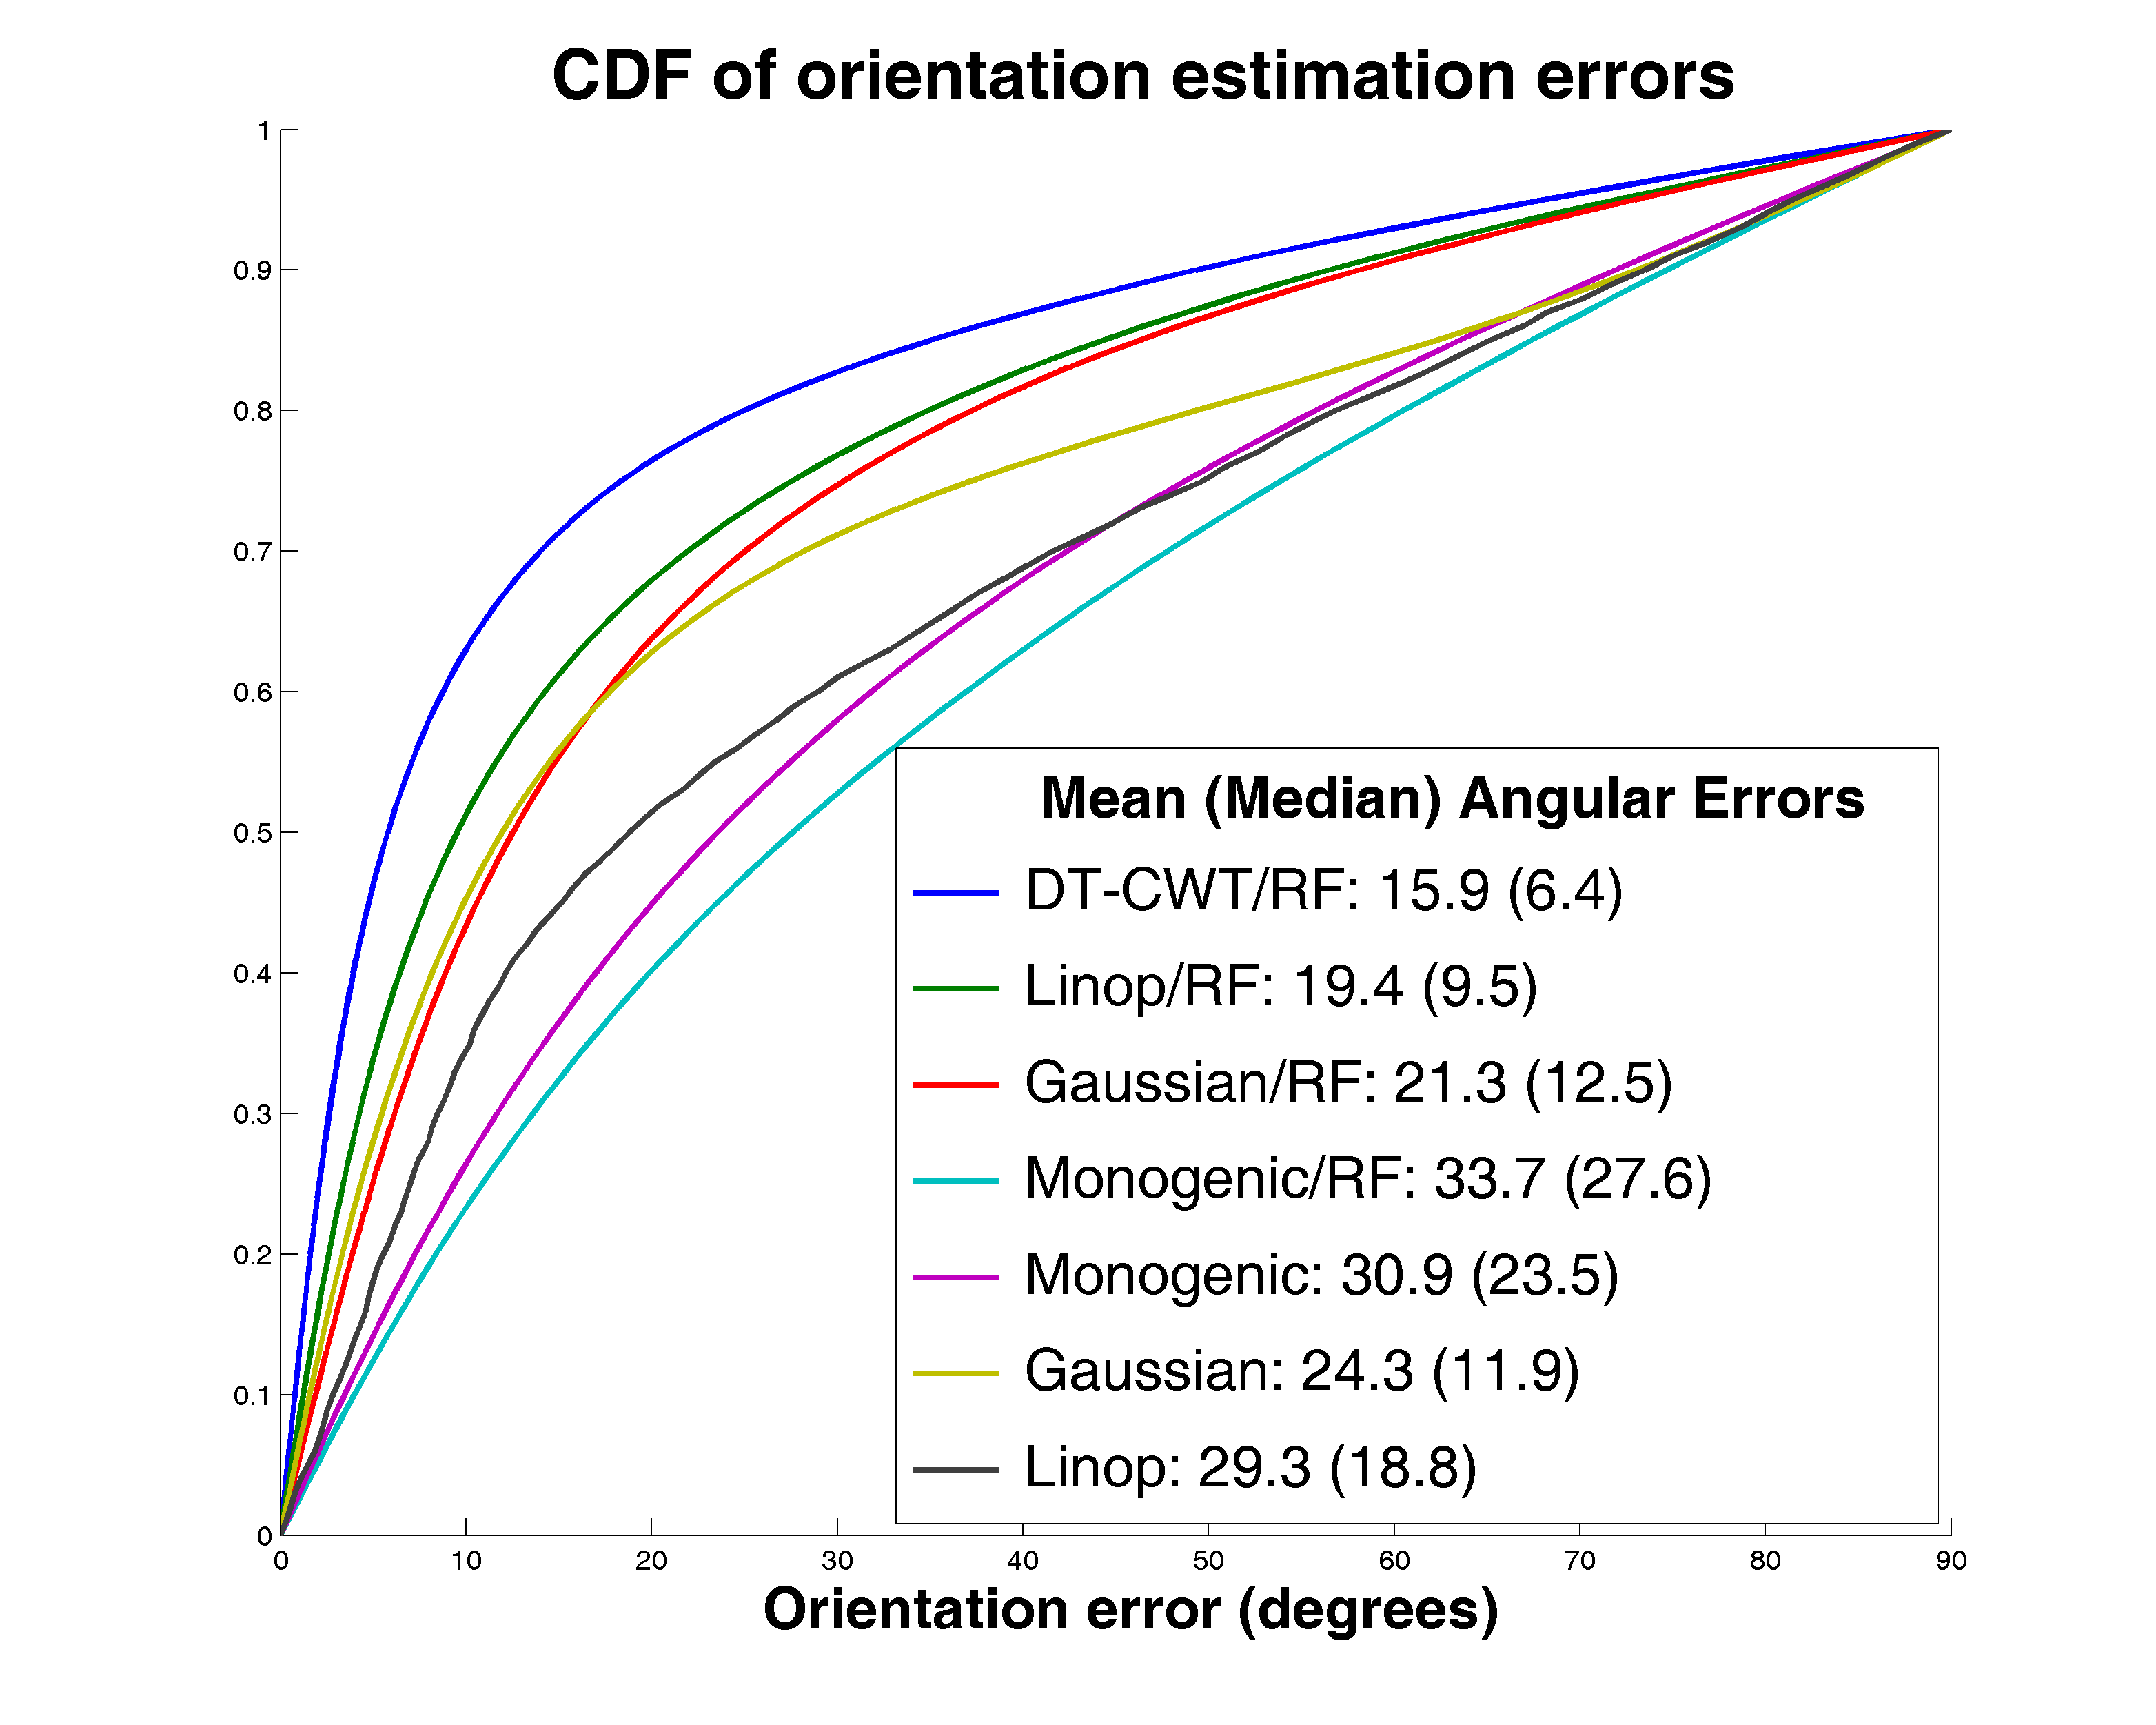
\includegraphics[width=0.33\columnwidth]{\figpath/ipmi/orientation_estimation_cdf} &
\end{tabular}
\end{figure}

\begin{table}
\caption{Results for spicule classification. For every algorithm, we show the area under the ROC curve ($A_z$)}
\label{t:spicule_classification}
%
\begin{tabular}{l c}
Algorithm
		& ROC $A_z$ \\
\hline
\dtcwt{}/RF ($w$ = 1, $s$ = 6, all orientations)
		& 0.761$\pm$0.0034 \\
Monogenic/RF ($w$ = 1, $s$ = 5, 8 orientations)
		& 0.748$\pm$0.0035 \\
Gaussian/RF ($w$ = 1, $s$ = 5, $\sigma_{min}$ = 1)
		& 0.718$\pm$0.0037 \\
Linop/RF ($w$ = 1, $s$ = 5, $\lambda$ = 4)
		& 0.716$\pm$0.0037 \\
\end{tabular}
\end{table}

\begin{figure}
\centering
\begin{tabular}{c c}
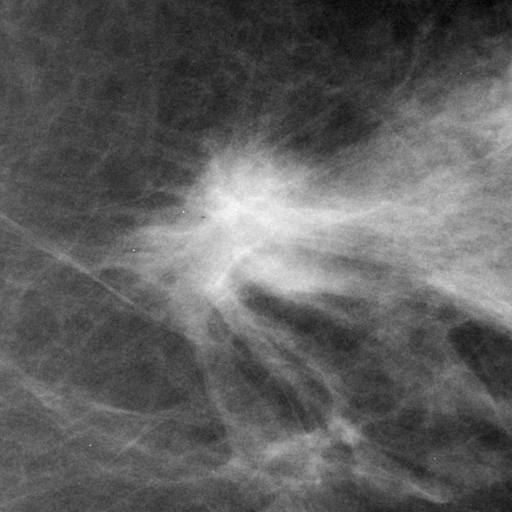
\includegraphics[width=\qtrcol]{\figpath/ipmi/mass046} &
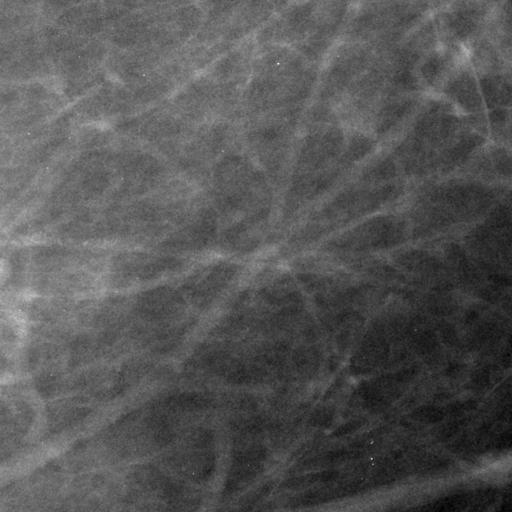
\includegraphics[width=\qtrcol]{\figpath/ipmi/norm068} \\
(a) & (b) \\
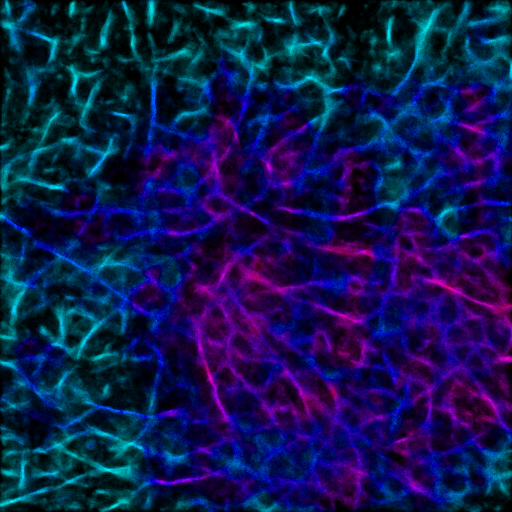
\includegraphics[width=\qtrcol]{\figpath/ipmi/spic_prob_mass046_a} &
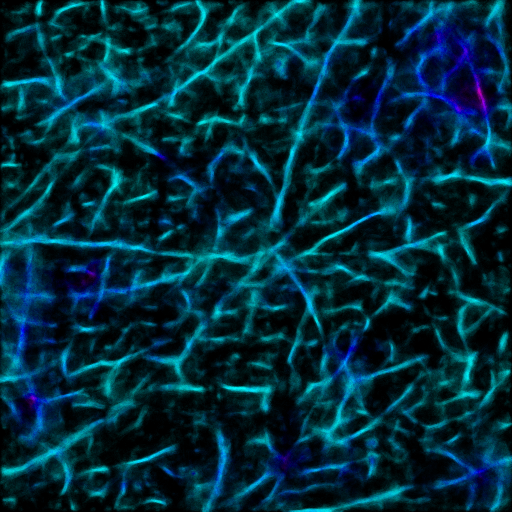
\includegraphics[width=\qtrcol]{\figpath/ipmi/spic_prob_norm068_a} \\
(c) & (d)
\end{tabular}
%
\caption{Regions depicting (a) malignant and (b) normal tissue. The corresponding spicule classification results are depicted in (c,d) using hue to indicate abnormality -- ranging from cyan (normal) to pink (spicule) -- and intensity to indicate the line detection output from the \dtcwt{} method.}
\label{f:spicule_classification}
\end{figure}


\section{Estimating Orientation}
In addition to detecting curvilinear structure in mammograms, for many subsequent analysis tasks (\eg~detecting abnormal patterns of structure indicative of disease) it is equally important that we can make accurate estimates of orientation. As with detection, rather than doing this prescriptively, we pose the problem as a regression task in which we learn how patterns of \dtcwt{} coefficients correspond to structures at varying orientations. Feature vectors of \dtcwt{} coefficients are formed as in section 2.1, with the difference that the image ground truth specifies the orientation of a pixel as opposed to its class membership. A random forest regressor can then be trained to predict the orientation of any pixel given its \dtcwt{} representation.

Curvilinear structures are important in many applications of computer vision, including aerial image analysis (roads, rivers, railways), fingerprint analysis (ridges) and medical image analysis (blood vessels, ducts). As a result, there is an extensive literature on detecting such structure~\cite{Papari_Petkov_IVC11}. The literature on estimating the local orientation of curvilinear structure is more limited though the problem is equally important, for example as a basis for non-maximal suppression (centre-line detection) and for characterising properties such as tortuosity (\eg~of blood vessels).

In mammography, malignant lesions often exhibit linear structures (known as spicules) that form a radial pattern around the central mass. Detecting linear structures and determining their orientation~\cite{Zwiggelaar_etal_MIA99,Zwiggelaar_etal_TMI04} can therefore indicate points where they converge and thus whether a mass or architectural distortion is present~\cite{Karssemeijer_teBrake_TMI96,Rangayyan_Ayres_MBEC06}. In other medical applications such as retinography (\fref{f:retinography}), the rate of change of orientation (\ie~tortuosity) of blood vessels can serve as a diagnostic indicator of vascular disease~\cite{Hart_etal_IJMI99}; though studies have shown that vessels can be detected and segmented~\cite{Staal_etal_TMI04,Ricci_Perfetti_TMI07,Dabbah_etal_MICCAI10}, few have addressed the problem of measuring their orientation and quantifying tortuosity.

Similarly, automatic fingerprint analysis typically begins by computing the orientation at each pixel via gradient-based filtering, often followed by some smoothing over a local patch~\cite{Bazen_Gerez_TPAMI02,Mei_etal_IVC09}. This orientation field is often parameterized -- via `phase portraits'~\cite{Li_etal_PR06} or polynomial approximation~\cite{Gu_etal_PR04}, for example -- to capture and interpret the underlying properties of the fingerprint such as its `singular points' where the orientation is no longer defined (\eg~at a delta or the centre of a whorl). Though smoothing orientation estimates at a local patch have been the subject of several investigations~\cite{Kass_Witkin_CVGIP87,Rao_Jain_TPAMI92,Perona_TIP98}, we deal only with the initial step of estimating orientation at every pixel.

In this paper we revisit the problem of orientation estimation, reviewing the basic theory, extending the state-of-the-art, and providing the results of extensive evaluation using both real and realistic synthetic images. The first step in estimating orientation usually involves applying a set of linear filters to the image, generally at multiple scales and orientations. As we will show later, the choice of filter-bank has a significant influence on both computational efficiency, and estimation accuracy. Our contribution is to explore the similarities and differences between different approaches, and provide empirical evidence of which work best in practice.

Given a set of filter-bank outputs, the second step in estimating orientation is to combine them in some way. There are two basic approaches: to find the scale at which the total magnitude of response is greatest, and combine the different filter responses at that scale analytically~\cite{Karssemeijer_teBrake_TMI96,Mei_etal_IVC09}; or to use a regression learning approach to combine the filter responses across all scales and orientations~\cite{Berks_etal_IPMI11}. Our contribution is to explore the technical details of orientation regression and provide a comprehensive evaluation of different combinations of filter-bank and analytic/regression methods. Overall we show that an approach based on combining dual-tree complex wavelet filtering with random forest regression achieves significantly better results than any of the other state-of-the-art approaches tested.

During testing, we applied each regressor in turn to estimate the orientation, $\theta_{est}$, at every pixel for every test image and computed the orientation error with respect to ground truth,
%
\begin{equation}
	\theta_{err} = \frac{\angle(2\theta_{est}-2\theta_{gt})}{2}
\end{equation}

\noindent only at labelled vessel pixels in the test image mask (\fref{f:retinography}c).\comment{A reviewer will probably complain that this is cheating and that we should have used a classifier}

These results show that the four learning methods perform significantly better than the three prescriptive methods (with the exception of orientation computation in Monogenic/RF). \dtcwt{}/RF is significantly the strongest performing for both line detection and orientation estimation, followed by Linop/RF then Gaussian/RF.

===

In our first set of experiments, we present a quantitative evaluation of the three regressors on real retinography images and mammogram-like data for which we have ground truth. We also present qualitative results on some real mammography images and fingerprint images for which ground truth was not available.


\subsection{Real Retinographic Images}
\label{s:expts_retinography}

\begin{table}[b]
\centering
\begin{tabular}{l|c c c c}
							& \multicolumn{4}{c}{Feature Type} \\
							& Monogenic		& 2nd deriv.	& Haar				& \dtcwt{} \\
\hline
\input{retinogram_table.txt}
\end{tabular}
%
\caption{Median absolute error (degrees) for combinations of input feature and regressor on the DRIVE database of retinal images (images 01-20).}
\label{t:retinopathy}
\end{table}

\begin{figure}
\centering
\begin{tabular}{c c}
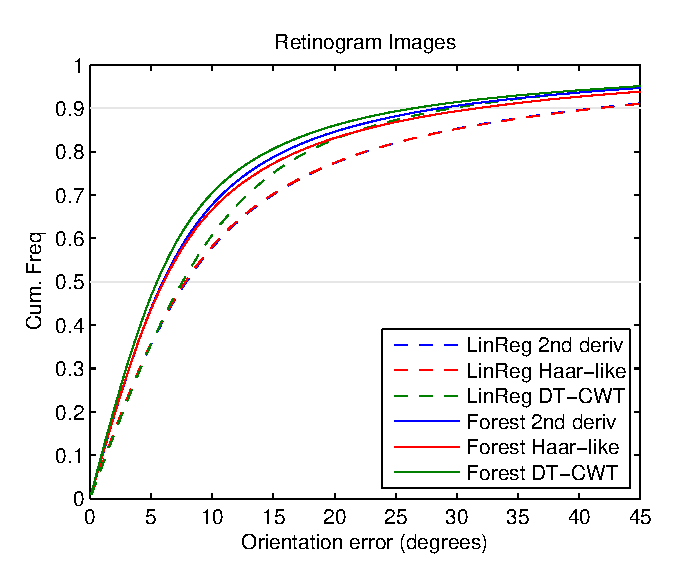
\includegraphics[width=0.48\columnwidth]{\figpath/retina/retinogram_expt} &
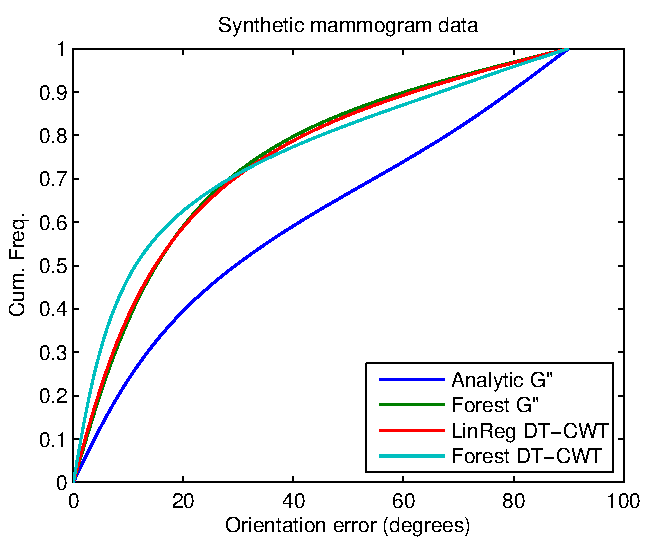
\includegraphics[width=0.48\columnwidth]{\figpath/mammo/mammography_expt} \\
(a) & (b) \\
\end{tabular}
%
\caption{Cumulative frequency of angular error for (a) retinogram images and (b) synthetic mammogram-like images.}
\label{f:cumfreq}
\end{figure}

Comparing performance for the various combinations (\fref{f:cumfreq}a and \tref{t:retinopathy}), we see that in general the analytic methods perform poorly in comparison with the regression approaches, that Random Forests outperform other regression methods and that the \dtcwt{} is superior to other feature representations. With the exception of the boosted regressor, the Haar-like approximation exhibited similar performance to the second derivative, suggesting that it may be used effectively in scenarios where efficiency is a concern.

It may be surprising just how poorly the analytic formulations perform in contrast to the regressors. On inspection of the outputs, we see that the monogenic signal (based on first derivatives) does indeed fail at the centre of linear structures. Since, however, many of the vessels in the retinograms are a single pixel in width (such that anywhere on the line is at the centre by definition) the monogenic signal is doomed. The regressors also get some benefit from pooling responses over several pixels.

As noted earlier, when using squared or second derivative responses it is necessary to compute the responses at the two possible solutions to determine which is the correct one. With the Haar-like approximation that combines the response to $\Ixx$ and $\Iyy$, this analytic solution is not available and a regression approach becomes necessary. Also, since the linear regressor minimizes the average error it contains no mechanism for selecting the correct orientation in this way. This is likely to be one reason for its poor performance relative to more sophisticated regressors such as the Random Forest. There is a penalty, however, in efficiency when using complex regressors like the Random Forest.


\subsection{Mammogram-like Images}
\label{s:expts_synth_mammography}
\begin{table}[t]
\centering
\begin{tabular}{l|c c c c}
							& \multicolumn{4}{c}{Feature Type} \\
							& Monogenic		& 2nd deriv.	& Haar				& \dtcwt{} \\
\hline
\input{mammography_table.txt}
\end{tabular}
%
\caption{Median absolute error (degrees) for combinations of input feature and regressor on 100 synthetic mammogram images.}
\label{t:synth_mammography}
\end{table}

As vessels are often clearly visible in retinograms, we repeated this experiment on a more challenging dataset of synthetic images that realistically approximate the structure of mammographic images. More specifically, we sampled a background by cropping a $512{\times}512$ image region from a real mammogram upon which we superimposed one or more lines of varying orientation, contrast, width and profile (\fref{f:synth_mammography}a). As the lines were synthetic, we had access to both a mask (\fref{f:synth_mammography}b) and ground truth orientation for the superimposed structure.

As in the retinogram experiment, we sampled 200\,000 pixels from such images and computed a feature vector for each with which we trained a regressor. We then applied every trained regressor for every feature type to a fixed set of 100 synthesized images and computed the error at the known foreground pixel positions (\fref{f:synth_mammography}c). As before, Random Forests and the \dtcwt{} outperform other methods, though errors were generally higher on account of the more challenging data (\fref{f:cumfreq}b and \tref{t:synth_mammography}). We also note that although the median error for the Random Forest was lower for the \dtcwt{} than the second derivatives, the situation was reversed for higher percentiles (\ie~the graphs cross). We care less, however, about differences between errors above a certain threshold (it matters little whether the estimate is out by $60^\circ$ or $70^\circ$ -- they are both terrible estimates) so it may be argued that the Random Forest performs better over the region in which we are interested.

\begin{figure}[t]
\centering
\begin{tabular}{c c c}
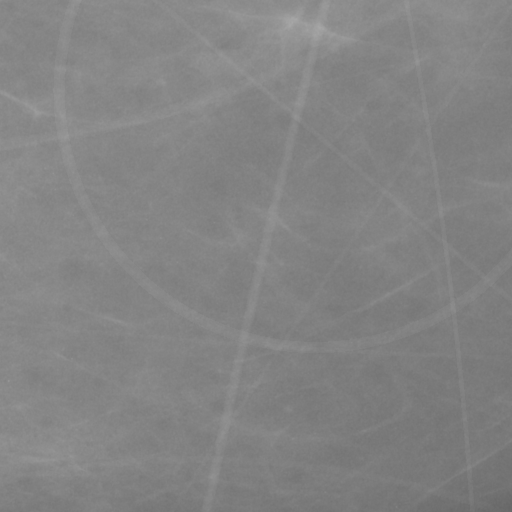
\includegraphics[width=0.3\columnwidth]{\figpath/mammo/synth_lines} &
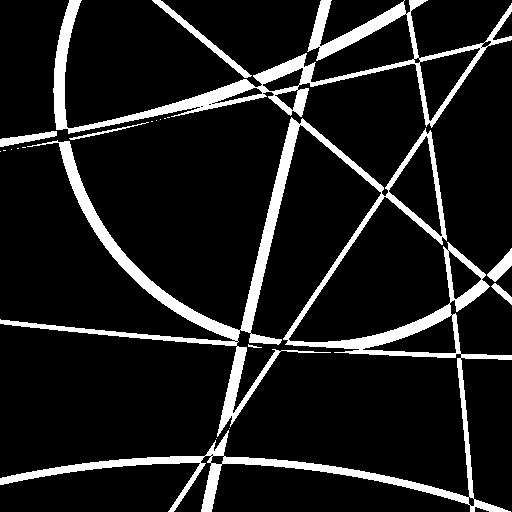
\includegraphics[width=0.3\columnwidth]{\figpath/mammo/synth_mask} &
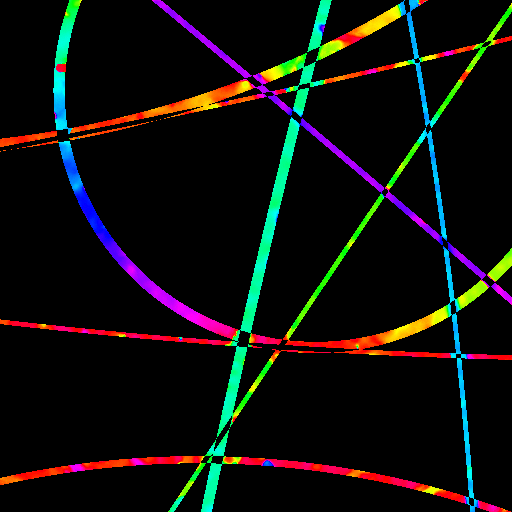
\includegraphics[width=0.3\columnwidth]{\figpath/mammo/synth_result} \\
(a) & (b) & (c)
\end{tabular}
%
\caption{Synthetic mammographic images: %
(a) input image; %
(b) mask indicating pixels belonging to a vessel; %
(c) orientation (indicated by colour) estimated using Random Forest regression over \dtcwt{} features. The mask was not used to estimate orientation.%
}
\label{f:synth_mammography}
\end{figure}

\begin{figure}[t]
\centering
\begin{tabular}{c c}
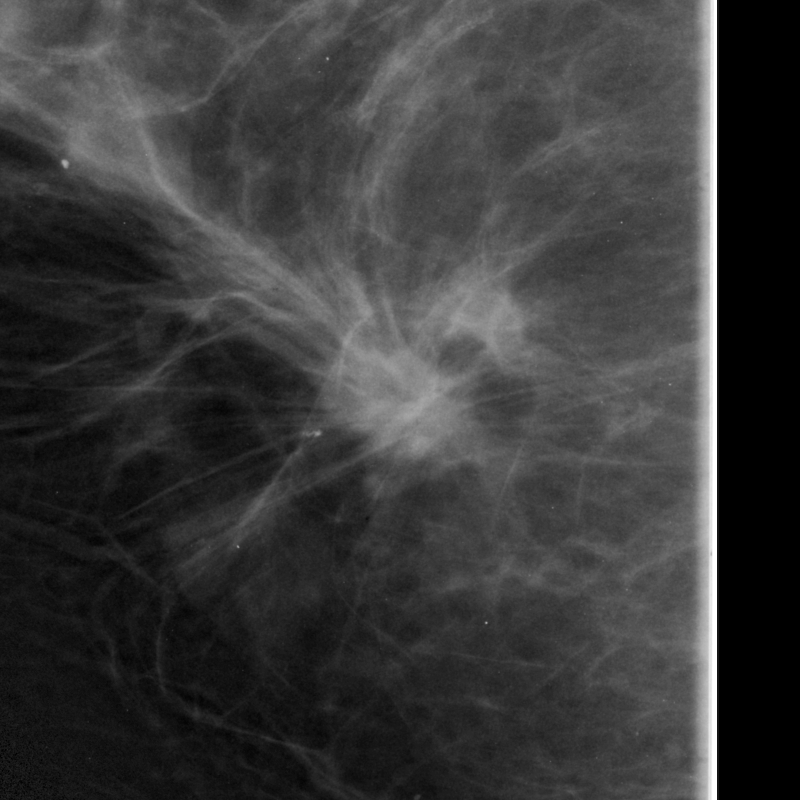
\includegraphics[width=0.3\columnwidth]{\figpath/mammo/024RCC_roi} &
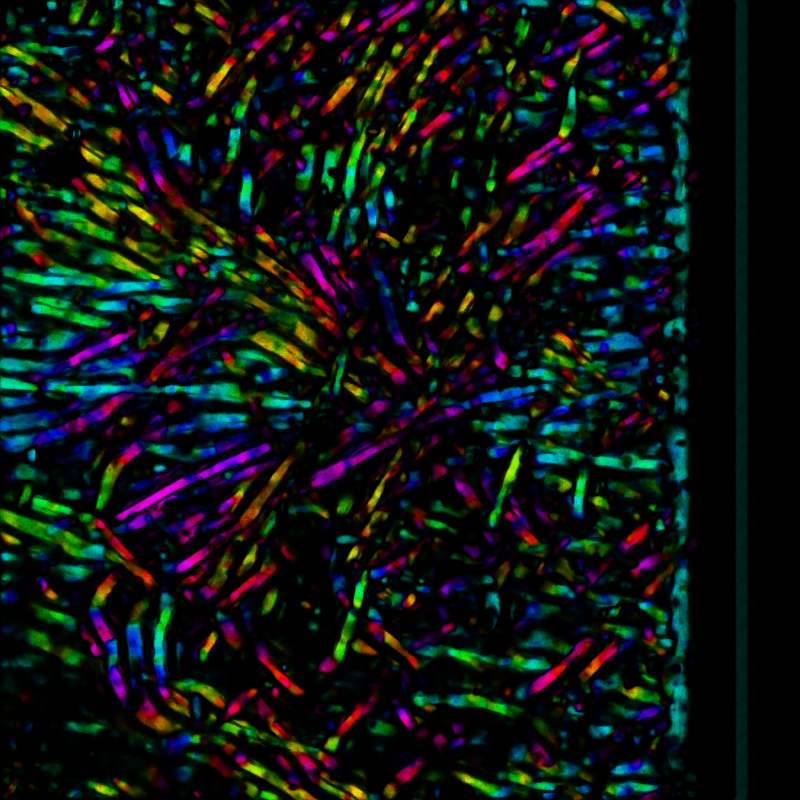
\includegraphics[width=0.3\columnwidth]{\figpath/mammo/024RCC_roi_class_ori_masked} \\
(a) & (b) \\
\end{tabular}
%
\caption{Real mammographic images: %
(a) input image; %
(b) estimated orientation from a Random Forest using \dtcwt{} features. Hue indicates the estimated orientation and brightness is determined by the confidence in the estimate (as quantified by the dispersion).}
\label{f:real_mammography}
\end{figure}

% CLAIM: that the separable filters are faster than nonseparable ones (but by how much?)
% CLAIM: that the Haar-like features are faster than separable filtering
In terms of efficiency, we recorded the mean time (using Matlab on a 2.66Ghz, quad-core desktop PC with 3.25Gb RAM) over 20 images for five feature representations: the monogenic signal (2.96\emph{s}); non-separable second derivatives (3.71\emph{s}); separable second derivatives (2.04\emph{s}); their Haar-like approximations (2.35\emph{s}); and the \dtcwt{} (19.96\emph{s}). Unsurprisingly, under test conditions the separable filters were indeed faster than their non-separable counterparts while the \dtcwt{} was an order of magnitude slower than the separable filters. The Haar-like approximations were comparable to but slower than the separable filters, though the separable filters did exploit the built-in (\ie~compiled) convolution functions in Matlab; we expect that an optimized implementation of the Haar-like features would offer similar performance gains as observed in face detection applications~\cite{Viola_Jones_IJCV04}.
%%% This is a pretty weak conclusion to the experiment but the best we can expect at this point. Also, if you need to use a regressor as slow as the RF to get accuracy that is comparable to the analytic second derivatives then the small difference in filtering time becomes irrelevant}

Having trained regressors on synthetic mammogram-like images, we can also apply them to real mammograms. In a region of interest surrounding a spiculated lesion, the linear structures radiating from the central mass are clearly visible when weighted by the confidence in their orientation estimation (\fref{f:real_mammography}).


\subsection{Fingerprint Analysis}
\label{s:expts_fingerprints}


\section{Discussion}
\label{s:discussion}
\begin{itemize}
\item Combining first and second derivatives: firsts are good at edges, seconds are good at line centres - they complement each other.

\item Discussion about linear regression coefficients: how they take a sinusoidal appearance, how we need to choose between two discrete orientations (which is not possible with a `vanilla' linear regressor)
%
\begin{figure}[t]
	\centering
		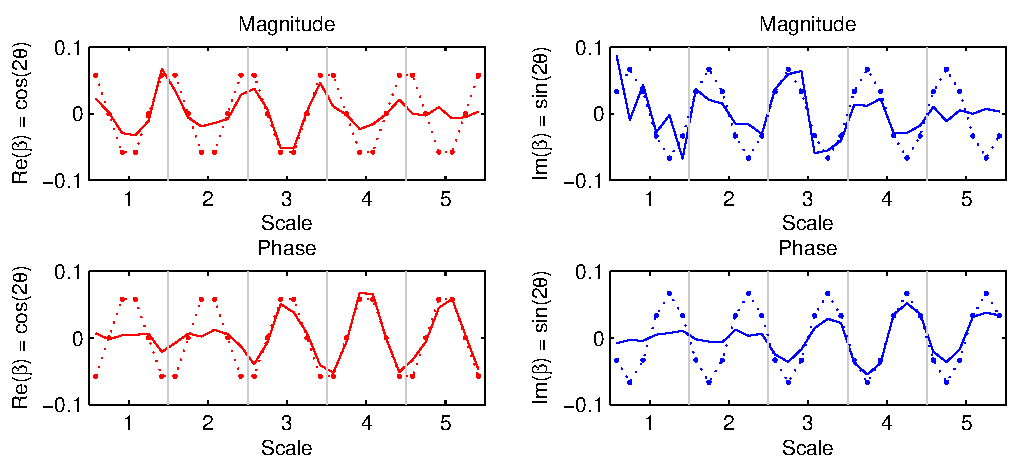
\includegraphics[width=0.9\columnwidth]{\figpath/linreg_coeffs}
	\caption{Linear regression coefficients for (left) $\cos 2\theta$ and (right) $\sin 2\theta$, using (top) response magnitude and (bottom) response phase.}
	\label{f:linreg_coeffs}
\end{figure}

\item Logistic regression can be used to limit the output to -1..+1. Boosted regression implicitly does the same by predicting only what it has seen before. These limits, however, are applied to sinT and cosT independently which means you can still get values outside of the unit circle.

\item Random Forest classifier/regressor has lots of details to get right, not least in making sure that the orientations wrap around correctly. Also differences in how the branches are split etc.

\end{itemize}

and orientation (the mean output of each regression tree, with appropriate angular wrapping at 0\deg and 180\deg) at each pixel

For orientation, only pixels belonging to curvilinear structures (although not necessarily at the centerline) were included in the results. The absolute differences between the predicted and known orientations (with appropriate angle wrapping) were taken, and used to generate cumulative distribution functions of orientation errors for each method, as shown in~\ref{f:}. The mean absolute errors of the estimated orientations are also included in~\ref{t:}.

The orientation results for both Monogenic and Monogenic/RF were surprisingly poor. Counter-intuitively, visual analysis of the test outputs showed that the Monogenic methods performed particularly badly at the exact centerline of curvilinear structures, where an essentially random orientation appeared to be returned. This is in contrast to the other tested methods that, as expected, performed strongest along the centerlines of structures. Computing estimation errors at pixels belonging to structures but not lying on the centerline produces a small improvement in the results (mean absolute errors of 32.55\deg and 29.39\deg for the RF and prescriptive variant respectively), though even then performance lags behind the other tested methods and of course in a real image we do not know the precise location of structure centerlines. Determining why orientations are estimated so poorly by the monogenic signal at the centre of structures, where in theory the signal is strongest, may warrant further investigation.




In terms of applying the learning methods to real images, it is worth noting how the methods scale with increasing image size - particularly above the point at which the set of feature vectors for all image pixels can be stored in working memory. For the \dtcwt{}, provided the initial decomposition can be stored in memory (which due to its low-redundant decimating construction is possible even for full size mammograms of the order 3000x2400 pixels) then interpolated coefficients can be efficiently sampled to generate feature vectors for block-wise regions of the image. Each block of feature vectors can be classified by the forest and cleared from working from memory storing only the output of the forest. In this way only a small overhead is introduced for block-wise classifying the image. However, for the other methods it becomes necessary to interleave the decomposition of the image with the sampling of feature vectors. For example, it may be necessary to apply the filters at a single scale, extract features for that scale for a particular block of the image, filter at the next scale and extract those features, and so on. Of course, when the complete feature vectors for a single block have been classified, the process repeats. Thus a large image may in fact end up by decomposed many times over introducing a large computational overhead for block-wise processing. The point at which this cost occurs will depend on the size of the image and the type of representation used. Obviously the cost is worst for Linop which requires storing 8 (\ie the number orientations) full copies of the image at each scale, compared to just 3 for the Gaussian and Monogenic methods.



\begin{table}
\centering
\caption{Line detection and orientation computation results. For every algorithm, we present the area under the ROC curve ($A_z$), the sensitivity at 90\% specificity, and the mean absolute error of the orientation estimate.}
\label{t:line_detection}
%
\begin{tabular}{l c c c}
Algorithm	
		& $A_z$							& Sens. \@ 90\% spec. & MAE \\
\hline
\dtcwt{}/RF ($w$ = 1, $s$ = 5)												
		& 0.923$\pm$0.00036	& 0.792 							& 15.88 \\
Linop/RF ($w$ = 1, $s$ = 5, 8 orientations)				
		& 0.911$\pm$0.00048	& 0.757								& 19.35 \\
Gaussian/RF ($w$ = 1, $s$ = 4, $\sigma_{min}$ = 1)
		& 0.901$\pm$0.00048	& 0.731								& 21.37 \\
Monogenic/RF ($w$ = 1, $s$ = 4, $\lambda$ = 4)
		& 0.868$\pm$0.00045	& 0.643								& 33.73 \\
Monogenic ($s$ = 3, $\lambda$ = 4)									
		& 0.818$\pm$0.00055	& 0.547								& 30.86 \\
Gaussian ($s$ = 4, $\sigma_{min}$ = 1)							
		& 0.813$\pm$0.00053	& 0.533								& 24.27 \\
Linop ($s$ = 5, 8 orientations)										
		& 0.737$\pm$0.00060	& 0.413								& 29.32 \\
\end{tabular}
\end{table}



\section{Discussion}
The results of our experimental evaluation are extremely encouraging, and represent a significant improvement over the current state of the art. 

Although learning accounts for a significant part of this improvement, the choice of representation is also important and will have a different effect on performance depending on the task in hand. For example, constructing a representation based on the raw responses to Linop filters produces features that are excellent for estimating structure orientation but provide less information for determining structure shape and thus type. 

Conversely, features formed from the monogenic signal are good at determining structure type - most likely because of the inclusion of the phase measure - while they perform relatively poorly at detection and orientation estimation. 

For these reasons, it seems fair to conclude that the \dtcwt{} provides the best all round representation. It produced the strongest performance for all three tasks (curvilinear structure detection, orientation estimation and spicule classification). Moreover, the \dtcwt{} incurs the least overhead when working with full-size real images that require block-wise classification/regression. For example, initial tests show that the structure detection and orientation regression can be performed on a full-size (~3000 x 2400 pixels) mammogram in ~1hr 30mins.

We show that, overall, our approach is significantly better than the current state-of-the-art, and that we can distinguish effectively between curvilinear structures associated with malignancy (spicules) and those associated with normal structure (vessels, ducts etc).